
%-----------------------------------------------------------------------------------
%	PACKAGES AND OTHER DOCUMENT CONFIGURATIONS
%----------------------------------------------------------------------------------



\documentclass[11pt]{article}

\usepackage[top=2cm, bottom=3cm, left=2cm, right=2cm]{geometry}

\setlength{\parindent}{0in}

\newcommand{\Var}{\mathrm{Var}}

\newcommand{\Cov}{\mathrm{Cov}}

\newcommand{\plim}{\rightarrow_{p}}

\usepackage{amsmath, amsfonts}
\usepackage{graphicx}
\usepackage{pdfpages}
\usepackage{bm}

% Expectation symbol
\newcommand{\E}{\mathrm{E}}
\newcommand{\V}{\mathrm{V}}

%----------------------------------------------------------------------------------
%	TITLE AND AUTHOR(S)
%----------------------------------------------------------------------------------

\title{Econ 675 Assignment 1} % The article title


\author{Nathan Mather} % The article author(s) 

\date{\today} % An optional date to appear under the author(s)


%----------------------------------------------------------------------------------
\begin{document}
	
%------------------------------------------------------------------------------
%	TABLE OF CONTENTS & LISTS OF FIGURES AND TABLES
%------------------------------------------------------------------------------
\maketitle % Print the title/author/date block

\setcounter{tocdepth}{2} % Set the depth of the table of contents to show sections and subsections only

\tableofcontents % Print the table of contents

\listoffigures % Print the list of figures

\listoftables % Print the list of tables
	
%-------------------------------------------------------------
% Question 1 
%-------------------------------------------------------------

\section{Question 1: Simple Linear Regression with Measurement Error}
\subsection{OLS estimator}
$\hat{\beta}_{ls} = (\tilde{x}'\tilde{x})^{-1}\tilde{x}'y$ and we want to show that $\hat{\beta}_{ls} 	\rightarrow_{p} \lambda\beta$
\\
\\
First note that
 
\begin{displaymath}
y=\beta(\tilde{x}-\mu)+\epsilon = \beta\tilde{x} + (\epsilon-\beta\mu)
\end{displaymath}

So The measurement error in $x$ becomes part of the error term in the regression. This means OLS will lead to a negative bias in $\hat{\beta}_{ls}$ if the true $\beta$ is positive and a positive bias in $\hat{\beta}_{ls}$ if the true $\beta$ is negative (an attenuation bias). In order to determine the magnitude of the bias consider the following. 

$$\hat{\beta}_{ls} = \frac{\mathrm{Cov}(\tilde{x},y)}{\mathrm{Var}(\tilde{x})}  
 = \frac{\mathrm{Cov}(x + \mu, \beta x + \epsilon )}{\mathrm{Var}(x + \mu)} 
 = \frac{\beta \Cov(x,x) + \Cov(x,\epsilon) + \Cov(\mu, \beta x) + \Cov(\mu, \epsilon)}{\Var(x + \mu)}$$
 
 $$ = \frac{\beta \Var(x) }{\Var(x + \mu)} \rightarrow_{p} \frac{\beta \sigma_{x}^2}{\sigma_{x}^2 + \sigma_{\mu}^2} = \lambda \beta$$
 
 $$\text{This implies that } \lambda = \frac{\sigma_{x}^2}{\sigma_{x}^2 + \sigma_{\mu}^2} $$
 
\subsection{Standard Errors}

Start with $ \hat{\epsilon} = y - \hat{\beta}_{ls}(x + \mu) $ \\
\\
 Now add and subtract the True error term $\epsilon = y - \beta x$ and collect terms to get $ \hat{\epsilon} + \epsilon - \epsilon = \epsilon - (y - \beta x) + y - \hat{\beta_{ls}} x - \hat{\beta}_{ls}\mu = \epsilon + (\beta - \hat{\beta}_{ls})x - \hat{\beta}_{ls} \mu$
 \\ \\
 recall that $\hat{\beta}_{ls} \rightarrow_{p} \lambda \beta $ and that $ \epsilon, x, \mu$ are all uncorrelated. This implies that $\hat{\sigma_{\epsilon}^2} \plim \sigma_{\epsilon}^2 + (1-\lambda)^2 \beta^2\sigma_{x}^2 + \lambda^2 \beta^2 \sigma_{\mu}^2$
 \\ \\ 
 so this is biased upwards since we are adding positive terms to the true value 
 \\ \\ 
 next to compute the probability limit of $\hat{\sigma}_{\epsilon}^2 (\tilde{x}'\tilde{x}/n)^{-1}$
 
 $$ \hat{\sigma}_{\epsilon}^2 (\tilde{x}'\tilde{x}/n)^{-1} = \frac{\hat{\sigma}_{\epsilon}^2}{\hat{\sigma}_{\tilde{x}}^2} \plim \frac{ \sigma_{\epsilon}^2 + (1-\lambda)^2 \beta^2\sigma_{x}^2 + \lambda^2 \beta^2 \sigma_{\mu}^2}{\sigma_{x}^2 + \sigma_{\mu}^2}$$
 
$$ =\frac{\sigma_{x}^2}{\sigma_{x}^2 + \sigma_{\mu}^2}(\frac{\sigma_{\epsilon}^2}{\sigma_{x}^2}) + \frac{\sigma_{x}^2}{\sigma_{x}^2 + \sigma_{\mu}^2}(1-\lambda)^2 \beta^2 + \frac{\sigma_{\mu}^2}{\sigma_{x}^2 + \sigma_{\mu}^2} \lambda^2 \beta^2  = \lambda(\frac{\sigma_{\epsilon}^2}{\sigma_{x}^2}) + \lambda (1-\lambda)^2 \beta^2 + (1-\lambda) \lambda^2 \beta^2  $$

now note that $  \lambda (1-\lambda)^2 \beta^2 + (1-\lambda) \lambda^2 \beta^2 = \beta^2\lambda (1-\lambda)[(1-\lambda) + \lambda] = \beta^2 \lambda (1-\lambda)$

Combining these gives us that 

$$ \frac{\hat{\sigma}_{\epsilon}^2}{\hat{\sigma}_{\tilde{x}}^2} \plim  \frac{\lambda \sigma_{\epsilon}^2}{\sigma_{x}^2} + \lambda(1-\lambda)\beta^2 $$

multiplying the first term by $\lambda$ biases the result downwards but the second term is positive so it biases the result upwards. So the overall result of the bias cannot be signed in general 

\subsection{t-test}

$$\frac{\hat{\beta}_{ls}}{\sqrt{\hat{\sigma}_{\epsilon}^2(\tilde{x}'\tilde{x}/n)^{-1}}} \plim \frac{\lambda \beta}{\sqrt{\lambda \frac{ \sigma_{\epsilon}^2}{\sigma_{x}^2} + \lambda(1-\lambda)\beta^2 }} 
= \frac{\sqrt{\lambda}\beta}{\sqrt{ \frac{ \sigma_{\epsilon}^2}{\sigma_{x}^2} + (1-\lambda)\beta^2 }}$$

which is smaller than 
$$ \frac{\beta}{\sqrt{\frac{\sigma_{\epsilon}^2}{\sigma_{x}^2}}}$$

So the t-test is downward biased 

\subsection{Second measurement, Consistency}

$$ y = x\beta + \epsilon$$


by assumption $ \E[\check{x} \epsilon] = 0 $ \\ 
Now multiply y by $ \check{x}'$ and take the expectation to get $ \E[\check{x}'y]=\E[\check{x}'x]\beta$ \\
Now assuming $\E[\check{x}'x]$ is full rank we get $\beta =(\E[\check{x}'x])^{-1}\E[\check{x}'y]$ \\
So $\hat{\beta}_{IV}=(\check{x}'x)^{-1}\check{x}'y$\\
Now to show it is consistent \\
$\hat{\beta}_{IV}=(\check{x}'x)^{-1}\check{x}'(x\beta  + \epsilon) = \beta + (\frac{\check{x}'x}{n})^{-1}(\frac{\check{x}'\epsilon}{n}) \plim \beta$ \\
since $\E[\check{x}'\epsilon] = 0$ so $\frac{\check{x}'\epsilon}{n} \plim 0$ by LLN

\subsection{Second measurement, Distribution}

$$\sqrt{n}(\hat{\beta}_{IV}-\beta) = (\check{x}'x)^{-1}\check{x}'\epsilon = \sqrt{n}\left(\frac{\check{x}'x}{n}\right)^{-1}\left(\frac{\check{x}'\epsilon}{n}\right)$$
Now using the CLT we get 
$$\sqrt{n}\left(\frac{\check{x}'\epsilon}{n}\right) \xrightarrow{d} N(0,\E[\check{x}'\epsilon'\epsilon\check{x}])$$
Now all together we get 
$$\sqrt{n}(\hat{\beta}_{IV}-\beta) \xrightarrow{d} N(0,\E[\check{x}'x]^{-1}\E[\check{x}'\epsilon'\epsilon\check{x}]E[x\check{x}']^{-1})$$

\subsection{Second measurement, Inference}
To create a confidence interval robust to Standard errors we want to use the following, unsimplified, version of the asymptotic variance estimator. 

$$\hat{V}_{IV} = Avar(\hat{\beta}_{IV}) = (\check{x}'x)^{-1}\left( \sum_{i=1}^{n}\epsilon_{i}^2 \check{x}_i' \check{x}_i \right) (\check{x}'x)^{-1}$$

We also showed above that 
$$
\sqrt{n}(\frac{\hat{\beta}_{IV}}{\sqrt{\hat{V}_{IV} }}) \to_d \mathcal{N}(\beta,1)
$$


Inverting the standard normal distribution and the following confidence interval 

$$ \left[ \hat{\beta}_{IV} - \Phi^{-1} \left( 1 -\frac{(1-\alpha)}{2} \right) \left( \sqrt{\frac{\hat{V}_{IV} }{n}} \right),  \hat{\beta}_{IV} + \Phi^{-1} \left( 1 -\frac{(1-\alpha)}{2} \right) \left( \sqrt{\frac{\hat{V}_{IV} }{n}} \right) \right] $$

where $\alpha = 0.95$ in this case 

\subsection{Validation sample, Consistency}

First note that $(\frac{1}{n}\tilde{x}'\tilde{x}) \plim \sigma_x^2 + \sigma_u^2$ and as shown in part 1 $\hat{\beta}_{ls} \plim \beta \frac{\sigma_{x}^2}{\sigma_{x}^2 + \sigma_{\mu}^2}$\\

Now we define $\hat{\beta}_{VS} = \hat{\beta}_{ls}\left(\frac{1}{n}\frac{\tilde{x}'\tilde{x}}{\check{\sigma}_x^2} \right)$ \\

and by Slutsky's theorem we get that $\hat{\beta}_{VS} \plim \beta$

\subsection{Validation sample, Distribution}

We know from section 1.7 that  $\hat{\beta}_{VS} = \hat{\beta}_{ls}\left(\frac{1}{n}\frac{\tilde{x}'\tilde{x}}{\check{\sigma}_x^2} \right)$ \\

We can break this into three pieces and define $\hat{\beta}_{VS}$ in the following way 

$$\hat{\beta}_{VS} = g(a,b,c) = \frac{ab}{c} $$
$$ a = \hat{\beta}_{ls} $$
$$ b = \frac{1}{n}\tilde{x}'\tilde{x} $$
$$ c = \check{\sigma}_x^2 $$

g is a continuous function so we can apply the delta method. 

$$ \sqrt{n} \left( g \left( \hat{\beta}_{ls}, \frac{1}{n}\tilde{x}'\tilde{x}, \check{\sigma}_x^2 \right) - g \left( \lambda \beta, \sigma_x^2 + \sigma_{\mu}^2, \sigma_x^2 \right) \right) \to_d 
\mathcal{N} \left( \nabla g \left( \lambda \beta, \sigma_x^2 + \sigma_{\mu}^2, \sigma_x^2 \right)' 
\bm{\Sigma} 
\nabla g \left( \lambda \beta, \sigma_x^2 + \sigma_{\mu}^2, \sigma_x^2 \right) \right) $$

$$ V_{vs} =  \nabla g \left( \lambda \beta, \sigma_x^2 + \sigma_{\mu}^2, \sigma_x^2 \right)' 
\bm{\Sigma} 
\nabla g \left( \lambda \beta, \sigma_x^2 + \sigma_{\mu}^2, \sigma_x^2 \right) $$

\subsection{Validation sample, Inference}

Similar to problem 1.6 we have that 
$$
\sqrt{n} \left( \frac{\hat{\beta}_{VS}}{\sqrt{\hat{V}_{VS} }} \right) \to_d \mathcal{N}(\beta,1)
$$


Inverting the standard normal distribution and the following confidence interval 

$$ \left[ \hat{\beta}_{VS} - \Phi^{-1} \left( 1 -\frac{(1-\alpha)}{2} \right) \left( \sqrt{\frac{\hat{V}_{VS} }{n}} \right),  \hat{\beta}_{VS} + \Phi^{-1} \left( 1 -\frac{(1-\alpha)}{2} \right) \left( \sqrt{\frac{\hat{V}_{VS} }{n}} \right) \right] $$

where $\alpha = 0.95$ in this case 

\subsection{FE estimator, Consistency}
First note that because we have $T=2$, the FE estimator is equivalent to the first-difference (FD) estimator. That is 


$$\hat{\beta}_{FE} = \hat{\beta}_{FD} $$
$$ \left( \frac{1}{n} \sum_{i-1}^{n}(\tilde{x}_{i2} - \tilde{x}_{i1} )^2 \right)^{-1} 
 \left( \frac{1}{n} \sum_{i-1}^{n}(\tilde{x}_{i2} - \tilde{x}_{i1} )(y_{i2}-y_{i1}) \right)$$
 
 Not by using the WLLN:
 
 $$ \frac{1}{n} \sum_{i-1}^{n}(\tilde{x}_{i2} - \tilde{x}_{i1} )^2 \plim \E[(\tilde{x}_{i2} - \tilde{x}_{i1} )^2]
  = \E[(x_{i2} - x_{i1} + u_{i2} - u_{i1})^2]$$
  $$ =  \E[(x_{i2} - x_{i1})^2] +\E[(u_{i2} - u_{i1})^2] +2\E[(x_{i2} - x_{i1})(u_{i2}-u_{i1})] = \sigma_{\Delta x}^2 + \sigma_{\Delta u}^2
  $$
  
  since $\E[x_{it}u_{it}] = 0$ $\forall$ $t,s \in \{1,2\}$ Next 
  
  $$\frac{1}{n} \sum_{i-1}^{n}(\tilde{x}_{i2} - \tilde{x}_{i1} )(y_{i2} - y_{i1}) \plim \E[(\tilde{x}_{i2} - \tilde{x}_{i1} )(y_{i2} - y_{i1})]$$
  
  $$ = \E[(x_{i2} - x_{i1} + u_{i2} -u_{i1})(x_{i2}\beta - x_{i1}\beta + e_{i2} - e_{i1})]$$
  
  $$ = \E[(x_{i2}-x_{i1})^2]\beta + \E[(x_{i2}-x_{i1})(e_{i2}-e_{i1})] + \E[(x_{i2}-x_{i1})( u_{i2} -u_{i1})]\beta + \E[(u_{i2} - u_{i1}(e_{i2} - e_{i1}))]
$$
$$ = \E[(x_{i2} - x_{i1})^2]\beta = \sigma_{\Delta x}\beta $$

since $\E[x_{it}u_{it}] = \E[x_{it}e_{it}] =  \E[u_{it}e_{it}] $ $\forall t,s \in \{1,2\}$. Finally we can put these together by the CMT to get. 
$$ \hat{\beta}_{FE} \plim \frac{\sigma_{\Delta x}^2}{\sigma_{\Delta x}^2 + \sigma_{\Delta u}^2} \beta
$$

Thus we can see that $\hat{\beta}_{FE}$ is biased downwards.

\subsection{FE estimator, time dependence}
Covariance stationarity implies that $\sigma_{xt}^2 = \sigma_x^2$ and $\sigma_{ut}^2 = \sigma_u^2$ for $t \in \{1,2\}$

this means that 
$$\sigma_{\Delta x}^2 =  \V[x_{i2} - x_{i1}] = \V[x_{i2}] + \V[x_i1] - 2Cov[x_{i2},x_{i1}] = 2\sigma_x^2 - 2Cov[x_{i2}, x_{i1}] $$

Thus we get 
$$\gamma = \frac{2(\sigma_x^2 - \Cov[x_{i2}, x_{i1}])}{2(\sigma_x^2 - \Cov[x_{i2}, x_{i1}] + \sigma_u^2 - \Cov[u_{i2}, u_{i1}])}$$

$$
= \frac{\sigma_x^2 - \rho_x \sigma_x^2 }{\sigma_x^2 - \rho_x \sigma_x^2 + \sigma_u^2 - \rho_u \sigma_u^2} = \frac{\sigma_x^2(1-\rho)x}{\sigma_x^2(1-\rho_x) + \sigma_u^2(1-\rho_u)} = \frac{\sigma_x^2}{\sigma_x^2 + \sigma_u^2 \frac{1-\rho_u}{1-\rho_x}}
$$

\subsection{FE estimator, time dependence}

let $\rho_u = 0$ given this we can calculate

$$ lim_{n\to\infty} \gamma = 0$$

This implies that under the given conditions $\hat{\beta}_{FE}$ will be biased to zero. Thus the FE estimator will tend to give you zero for coefficients regardless of the true $\beta$.
The idea is that if x is almost perfectly correlated over time, but the measurement error is completely random, then the only variation in our observations over time is because of random measurement error. So, our ability to observe actual variation in the variable of interest x is going to zero and the level of noise in our observations is high. 



\section{Question 2: Implementing Least-Squares Estimators}

\subsection{part 1}

Start by adding and subtracting $x \tilde{\beta}$ to get 
$$ (y-x\tilde{\beta} + x\tilde{\beta} - x\beta)'W(y-x\tilde{\beta} + x\tilde{\beta} - x\beta) $$
$$ = (y-x\tilde{\beta})'W(y-x\tilde{\beta}) + (y-x\tilde{\beta})'W(x\tilde{\beta} - x\beta) + (x\tilde{\beta} - x\beta)'W(y-x\tilde{\beta}) + (x\tilde{\beta} - x\beta)'W(x\tilde{\beta} - x\beta)$$
$$ = (y-x\tilde{\beta})'W(y-x\tilde{\beta}) + 2(x\tilde{\beta} - x\beta)'W(y-x\tilde{\beta}) + (x\tilde{\beta} - x\beta)'W(x\tilde{\beta} - x\beta)$$

Now we need to find $\tilde{\beta}$ to minimize this equation. We want to set the middle term to zero so we need a $\tilde{\beta}$ such that $\tilde{\beta}'x'W(y-x\tilde{\beta}) = \beta'x'W(y-x\tilde{\beta})$
\\ \\ 
we pick $\tilde{\beta}$ such that $x'W(y-x\tilde{\beta}) = 0$ giving us $$\tilde{\beta}=(x'W'x)^{-1}(x'Wy)$$

Now when we minimize over $\beta$ the first term is irrelevent as it does not include a $\beta$. The middle term is 0 so it does not matter. The last term is positive semi definite and so it is minimized by setting $\beta = \tilde{\beta}$

\subsection{Part 2}

$$ \sqrt{n} (\hat{\beta}(w)- \beta) = \sqrt{n}((x'Wx)^{-1}x'W(x\beta+\epsilon)-\beta)  
= \sqrt{n}((x'Wx)^{-1}x'W \epsilon)$$ \\
$$ = ((\frac{1}{n}x'Wx)^{-1} \sqrt{n} (\frac{1}{n} x'W\epsilon))$$

under appropriate assumptions we have by LLN that $ (\frac{1}{n}x'Wx) \plim A $ \\
We also have that $  \sqrt{n} (\frac{1}{n} x'W\epsilon) \rightarrow_{d} \mathcal{N}(0,B)$ by CLT  \\
In this case we get $ B = \frac{1}{n}  \mathbb{V}[x'W\epsilon] = \frac{1}{n} \mathbb{E}[x'W\epsilon'\epsilon Wx] $\\
And we have that $ V(W) = A^{-1}BA^{-1} $
 
\subsection{Part 3}

To estimate $V(W) = A^{-1}BA^{-1} $ we are mostly just putting hats on things 

$$\hat{A} = \frac{1}{n}(x'\hat{W}x)$$ 
$$\hat{B} = \frac{1}{n}(x'\hat{W} \hat{\epsilon}' \hat{\epsilon} \hat{W}x)$$

 so that gives us 
 
 $$ \hat{V}(W) = \frac{1}{n} (x'\hat{W}x)^{-1} (x'\hat{W} \hat{\epsilon}' \hat{\epsilon} \hat{W}x) (x'\hat{W}x)^{-1} $$
 
 \subsection{Part 4}
 
 See code in the appendix. The results do not change between the regular and Cholesky inverse. 
 
  \subsection{Part 5}
  
 	\subsubsection{a}
 	\begin{center}
 		% latex table generated in R 3.3.2 by xtable 1.8-2 package
% Thu Sep 27 20:51:41 2018
\begin{tabular}{rrrrrr}
  \hline
beta & se & t\_test & p\_value & CI\_L & CI\_U \\ 
  \hline
6485.55 & 4513.51 & 1.44 & 0.15 & -2384.89 & 15356.00 \\ 
  1535.48 & 638.24 & 2.41 & 0.02 & 281.15 & 2789.82 \\ 
  -2592.38 & 795.00 & -3.26 & 0.00 & -4154.80 & -1029.96 \\ 
  39.34 & 40.47 & 0.97 & 0.33 & -40.20 & 118.88 \\ 
  -740.54 & 944.68 & -0.78 & 0.43 & -2597.13 & 1116.05 \\ 
  60.08 & 53.77 & 1.12 & 0.26 & -45.59 & 165.75 \\ 
  -0.03 & 0.10 & -0.29 & 0.77 & -0.23 & 0.17 \\ 
  0.18 & 0.13 & 1.33 & 0.18 & -0.08 & 0.43 \\ 
  1316.03 & 1505.93 & 0.87 & 0.38 & -1643.58 & 4275.64 \\ 
  -1167.69 & 1275.42 & -0.92 & 0.36 & -3674.27 & 1338.90 \\ 
   \hline
\end{tabular}

 	\end{center}
 
 	\subsubsection{b}
 	They coincide because I made sure to weight the variance matrix properly and used HC1 in the sandwich package in R
 		\begin{center}
 		% latex table generated in R 3.3.2 by xtable 1.8-2 package
% Thu Sep 27 20:51:42 2018
\begin{tabular}{lrrrr}
  \hline
term & estimate & std.error & statistic & p.value \\ 
  \hline
(Intercept) & 6485.55 & 4513.51 & 1.44 & 0.15 \\ 
  treat & 1535.48 & 638.24 & 2.41 & 0.02 \\ 
  black & -2592.38 & 795.00 & -3.26 & 0.00 \\ 
  age & 39.34 & 40.47 & 0.97 & 0.33 \\ 
  educ & -740.54 & 944.68 & -0.78 & 0.43 \\ 
  educ\_sq & 60.08 & 53.77 & 1.12 & 0.26 \\ 
  earn74 & -0.03 & 0.10 & -0.29 & 0.77 \\ 
  black\_earn74 & 0.18 & 0.13 & 1.33 & 0.18 \\ 
  u74 & 1316.03 & 1505.93 & 0.87 & 0.38 \\ 
  u75 & -1167.69 & 1275.42 & -0.92 & 0.36 \\ 
   \hline
\end{tabular}

 	\end{center}
 	
 
 \section{Question 3: Analysis of Experiments}
 
 
 \subsection{Neyman's approach}
 
 \subsubsection{a}
 
 $$\E[T_{DM}] = \E[\bar{Y}_1] - \E[\bar{Y}_0] = \E \left[ \frac{1}{N_1} \sum_{i=1}^{n} D_i(1) Y_i  \right]  
 -  \E \left[ \frac{1}{n-N_1} \sum_{i=1}^{n} D_i(0) Y_i  \right]  $$
 
 $$ =  \frac{1}{N_1} \sum_{i=1}^{n} \left(  D_i(1) \E[Y_i] \right) - \frac{1}{n-N_1} \sum_{i=1}^{n} \left(  D_i(0) \E[Y_i] \right) $$
 $$=  \frac{1}{N_1} \sum_{i=1}^{n} \left( D_i(1) \right) \E[Y_i(T_i)|T_i = 1]  - \frac{1}{n-N_1} \sum_{i=1}^{n} \left( D_i(0) \right) \E[Y_i(T_i)|T_i =0] $$
 
 Now note that since $T_i$ is random: 
 $$ \E[Y_i(T_i)|T_i = 1] = \E[Y_i(1)] $$
 $$ \E[Y_i(T_i)|T_i = 0] = \E[Y_i(0)] $$
 
 Together this gives us: 
  $$\E[T_{DM}] = \E[Y_i(1)] - \E[Y_i(0)] $$
  
 or
 
 $$\tau_{ATE} = \frac{1}{n} \sum_{i=1}^{n} Y_i(1) - \frac{1}{n} \sum_{i=1}^{n} Y_i(0) $$
 
 The estimate from the data is 1794.34 and can be seen in the table in part 2
 
  \subsubsection{b}
 
 \begin{center}
 	% latex table generated in R 3.3.2 by xtable 1.8-2 package
% Thu Sep 27 22:25:40 2018
\begin{tabular}{rrrr}
  \hline
TDM est & Conservative SE & CI Lower & CI Upper \\ 
  \hline
1794.34 & 671.00 & 479.21 & 3109.47 \\ 
   \hline
\end{tabular}

 \end{center}
 
 \subsection{Fisher's approach}
 \subsubsection{a}
 
  \begin{center}
 	% latex table generated in R 3.3.2 by xtable 1.8-2 package
% Thu Sep 27 22:25:40 2018
\begin{tabular}{r}
  \hline
DM P value \\ 
  \hline
0.01 \\ 
   \hline
\end{tabular}

 \end{center}
  \begin{center}
	% latex table generated in R 3.3.2 by xtable 1.8-2 package
% Thu Sep 27 22:25:40 2018
\begin{tabular}{r}
  \hline
KS P value \\ 
  \hline
0.04 \\ 
   \hline
\end{tabular}

  \end{center}
 \subsubsection{b}
 To find the confidence interval I calculate fisher's exact P value for a range of Null hypotheses. The table for this calculation is below. We can then look the table and look for p values closest to our .05 cutoff. This gives us a confidence interval of 500 to 3000. Using a more detailed set of points I can find that the confidence interval is more precisely 540 to 3055.
 \begin{center}
 	% latex table generated in R 3.3.2 by xtable 1.8-2 package
% Thu Sep 27 20:51:42 2018
\begin{tabular}{rr}
  \hline
hyp\_treat & p\_value \\ 
  \hline
5000.00 & 0.00 \\ 
  4750.00 & 0.00 \\ 
  4500.00 & 0.00 \\ 
  4250.00 & 0.00 \\ 
  4000.00 & 0.00 \\ 
  3750.00 & 0.00 \\ 
  3500.00 & 0.01 \\ 
  3250.00 & 0.02 \\ 
  3000.00 & 0.06 \\ 
  2750.00 & 0.14 \\ 
  2500.00 & 0.25 \\ 
  2250.00 & 0.50 \\ 
  2000.00 & 0.73 \\ 
  1750.00 & 0.95 \\ 
  1500.00 & 0.64 \\ 
  1250.00 & 0.39 \\ 
  1000.00 & 0.20 \\ 
  750.00 & 0.08 \\ 
  500.00 & 0.05 \\ 
  250.00 & 0.01 \\ 
  0.00 & 0.01 \\ 
  -250.00 & 0.00 \\ 
  -500.00 & 0.00 \\ 
  -750.00 & 0.00 \\ 
  -1000.00 & 0.00 \\ 
  -1250.00 & 0.00 \\ 
  -1500.00 & 0.00 \\ 
   \hline
\end{tabular}

 \end{center}
 
 \subsection{Power calculations}
 \subsubsection{a}
 
\begin{minipage}{\linewidth}
	\begin{center}
		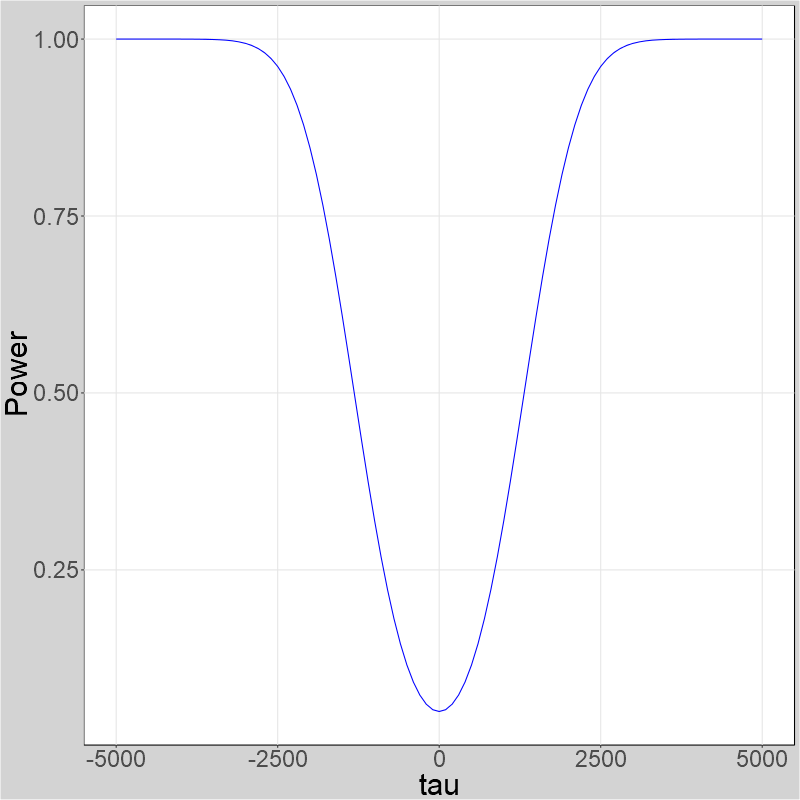
\includegraphics[width=.6\linewidth]{power_func_r.png}
	\end{center}
\end{minipage}




 \subsubsection{b}
 The math can be seen in my code. The number required is 1437
 
 \section{Appendix}
 \subsection{R Code}
 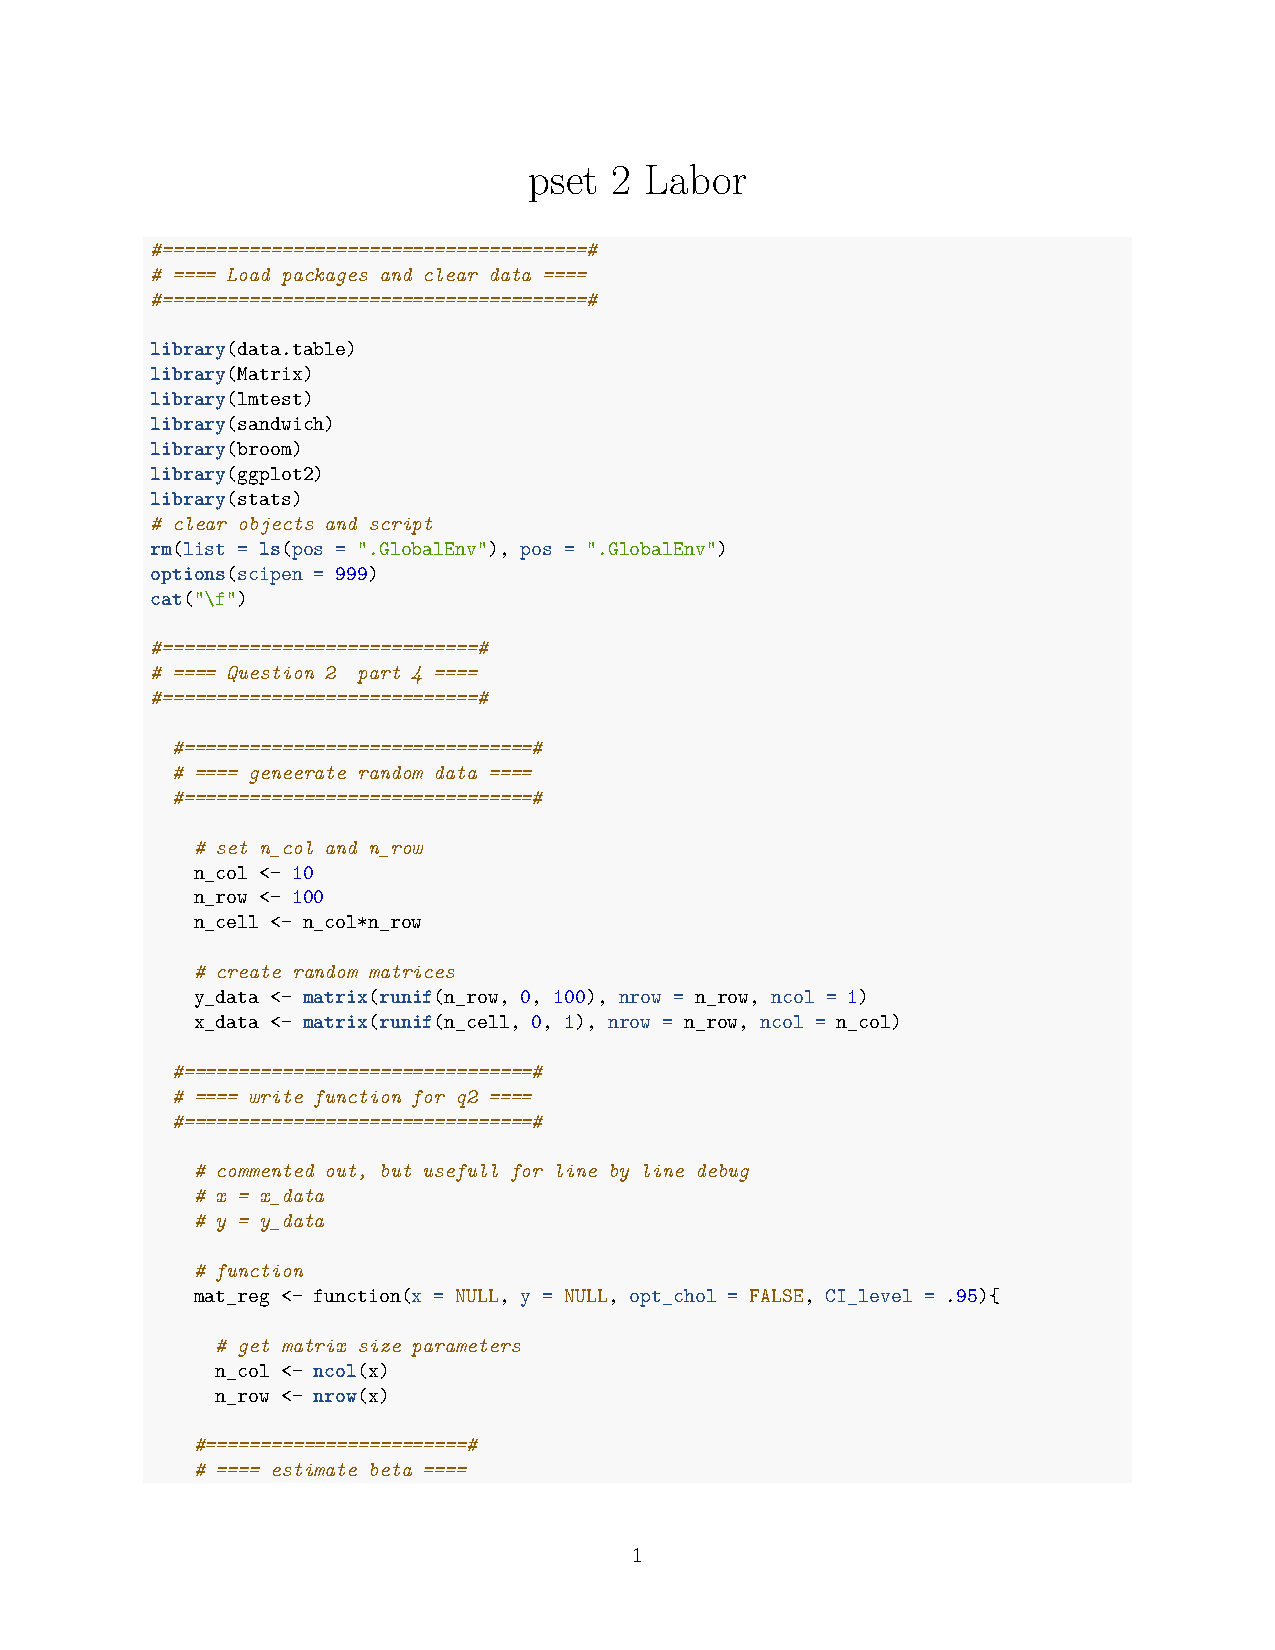
\includepdf[page=-]{assignment_1_r_code_pdf.pdf}
 
 \subsection{Stata Code}
  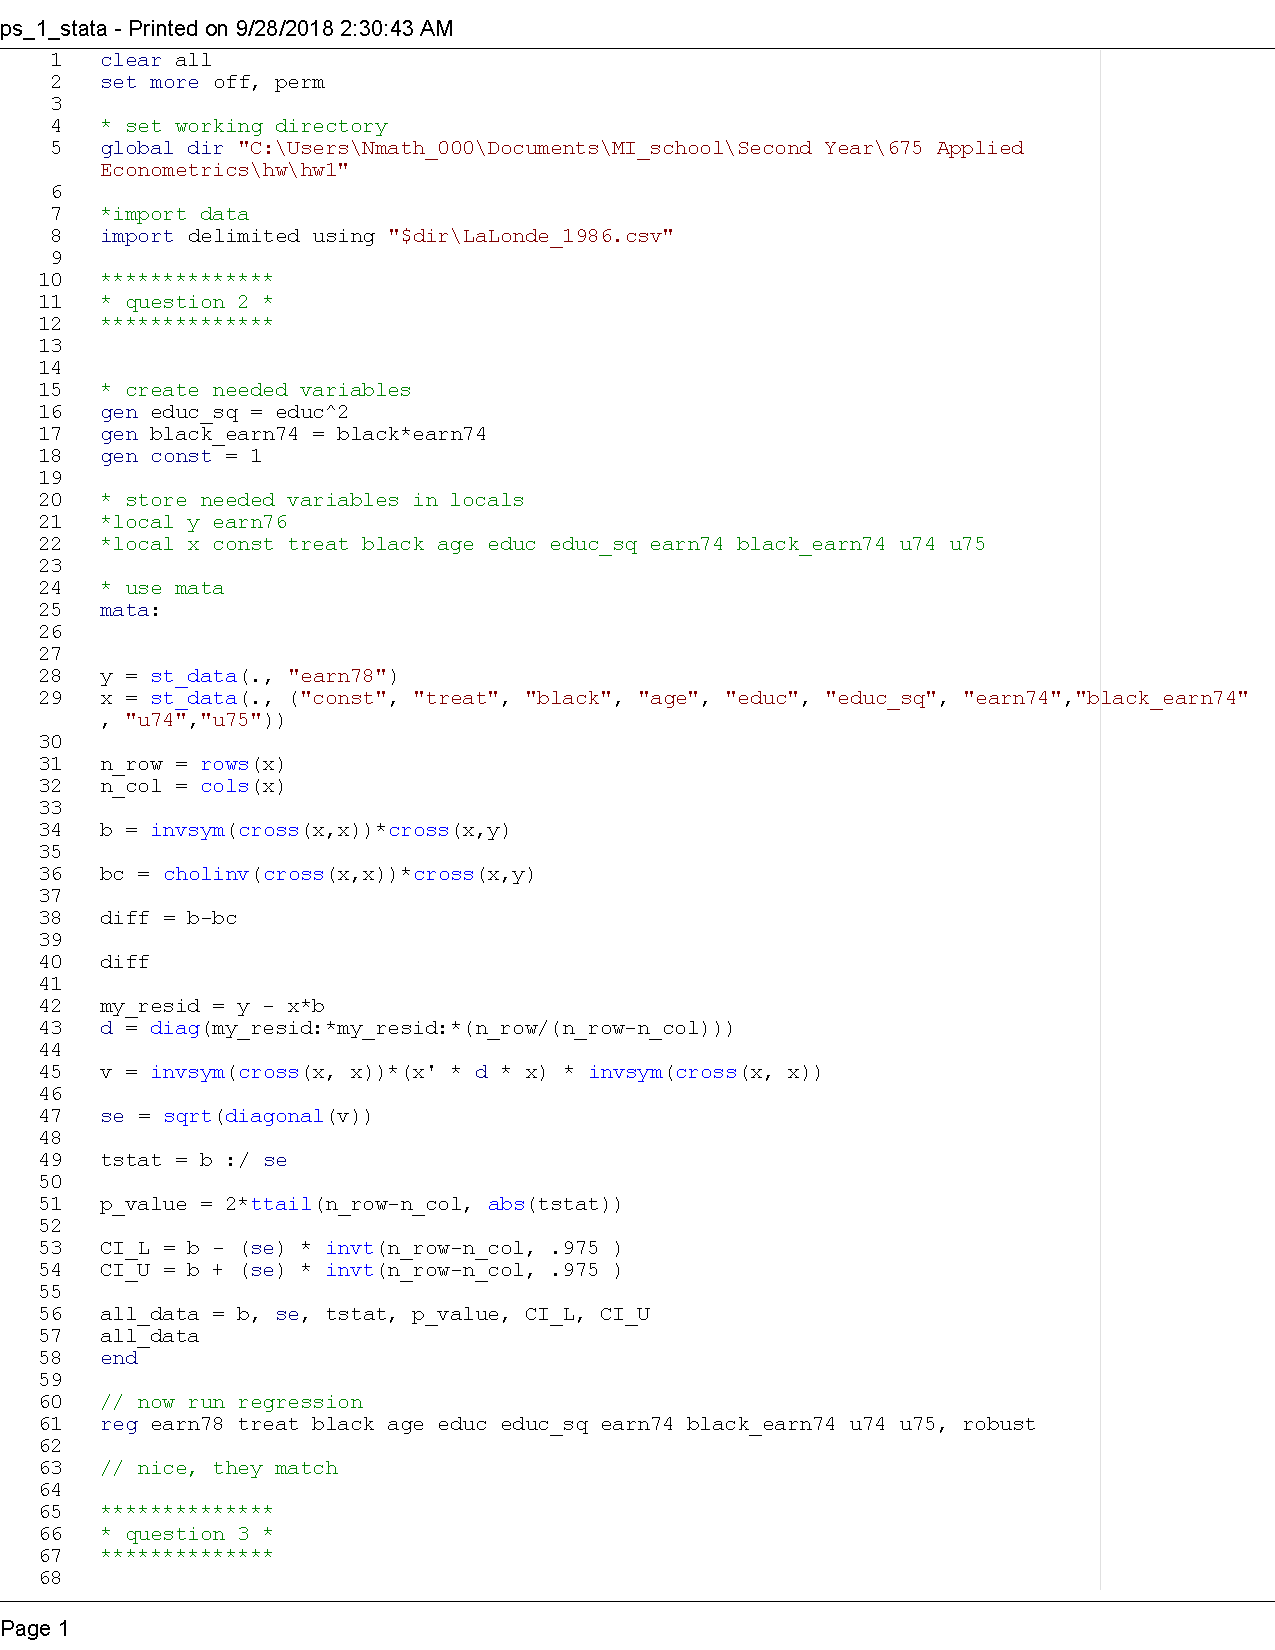
\includepdf[page=-]{assignment_1_stata_code_pdf.pdf}
 
 
%------------------------------------------------
% end doc
%------------------------------------------------
\end{document}



